\documentclass[12pt]{article}

\usepackage{fullpage}
\usepackage{graphicx}
\usepackage{graphics}
\usepackage{mdwlist}


% christos: these look closer to NSF specs\dots
\setlength{\oddsidemargin}{0.0in}
\setlength{\evensidemargin}{0.0in}
\setlength{\textwidth}{6.5in}
\setlength{\headheight}{0.0in}
\setlength{\topmargin}{0.0in}
% \setlength{\textheight}{9.0in}
\setlength{\textheight}{9in}
\addtolength{\textheight}{-\topmargin}
\addtolength{\textheight}{-\headheight}
\addtolength{\textheight}{-\headsep}
\addtolength{\textheight}{-\footskip}



\begin{document}

\newcommand{\beq}{\begin{equation}}
\newcommand{\eeq}{\end{equation}}
\newcommand{\bit}{\begin{itemize*}}
\newcommand{\eit}{\end{itemize*}}
\newcommand{\goal}[1]{ {\noindent {$\Rightarrow$} \em {#1} } }
\newcommand{\hide}[1]{}
\newcommand{\comment}[1]{ {\footnotesize {#1} } }
\newtheorem{lemma}{Lemma}
\newtheorem{theorem}{Theorem}
\newtheorem{proof}{Proof}
\newtheorem{defn}{Definition}
\newtheorem{algo}{Algorithm}
\newtheorem{observation}{Observation}

\title{Catchy Title}


\author{ {\em John Smith} \\
	    Dept. of Computer Science \\
	    CMU\\
	    {\tt jsmith@cs.cmu.edu}
	 \and
	 {\em Mary Thompson} \\
	     Dept. of Biology \\
	     Univ. of Pittsburgh\\
	     {\tt mj@upitt.edu}
	 \and
	 {\em Michael Miller} \\
	      Dept. of Physics \\
	      CMU
	      {\tt mm@andrew.edu}
        }


\maketitle
\begin{abstract}
    How similar are two sound-clips?
what is the best rhetorical question you can ask?
In this project, we develop {\em SomeMETHOD},
a fast and effective way of measuring the similarity
between two short sound clips.

\end{abstract}

\section{Introduction}
    \label{sec:intro}
    % {\em
% \bit
% \item
% what is the problem
% \item
% what are the applications
% \eit
% }

The basic idea of inference problem is try to get something interesting based on 
the observation and some probability constrains.
For example, given the constrains on the original code and the noisy channel's property, how can we get the original code from the received corrupted code.

\subsection{Pairwise MRF}
Pairwise Markov Random Field is a useful tool to model the inference problem where constrains only happens between two facts.

It provides a graph view of the problem.
The observation are known nodes in the graph and the information we want are unknown nodes.
The internal constrains between observation and corresponding information are modeled as an edge between known nodes and unknown nodes.
And the constrains, or compatibility, between two facts are expressed as an edge connecting the two unknown nodes.

Factor Graphs, Potts model and Bayesian Networks are some other models for inference problem.
As showed by Yedidia\cite{Yedidia:2003:UBP}, all these models can be converted into pairwise MRF model.

\subsection{Belief Propagation}
Based on the pairwise MRF graph, there is a message passing algorithm to compute the marginal possibility of unknown nodes.

The messages are defined like this: ``I think the chance that you are in state x is p".
It's expressed as $m_{ij}(x_j)$, which is the chance that node i thinks node j is in state $x_j$.

If we know the state of node i is $x_i$, then we can simply get $m_{ij}(x_j) \equiv \psi(x_i, x_j)$, where $\psi(x_i, x_j)$
is the constrain between information i and information j.

Apply the information of what other unknown nodes think node i is into the $m_{ij}(x_j)$ we just get via complete probability formula, the result would be
$$m_{ij}(x_j) \equiv \sum_{x_i} {\psi(x_i, x_j) \prod_{k \in N(x_i) \backslash j}{m_{ki}(x_i)}}$$

Gather the internal constrains between the observation and information i, we can get
$$m_{ij}(x_j) \equiv \sum_{x_i} {\phi(x_i) \psi(x_i, x_j) \prod_{k \in N(i) \backslash j}{m_{ki}(x_i)}}$$

This is exactly how Belief Propagation defines the message and the update of messages\cite{UBP}. And the final probability of information i is $x_i$ would be(k is used for normalization):
$$b_i(x_i) \equiv k\phi(x_i)\prod_{j \in N(i)} m_{ji}(x_i)$$

\subsection{Fast Algorithm for Belief Background}
The original Belief Propagation (\textbf{BP}) is essentially a message passing algorithm on the graph model depicting the dependency relationships among all nodes (variables or events) we care about. The great idea inside this algorithm is to achieve a complicate computation result by aggregating many local simple calculations. It breaks the marginal probability computation, the number of whose product terms increases exponentially with respect to the number of random variables, into linear number of local computations on every node. which has been discussed in previous sections.

One one hand, The message passing scheme makes the computation flow quite clear and understandable. One the other hand, the general mathematical expression for \textbf{BP} is not transparent now, for the whole computation is divided into many small local message calculations for every node. It is not very convenient and easy to convert the message flow into one or several highly summarized mathematical formulas. Since \textbf{BP} has the typical message generating and passing scheme, a variety of message schedules can be used to solve it in a finite number of steps. This also means that the message schedule solution dominates the efficiency of \textbf{BP}.

\subsection{Problem}

The problems we want to solve is the following:
\bit
\item GIVEN: the BP algorithm
\item FIND: a way to run it on hadoop
\item TEST: on some data sets with more than 2 states per nodes
\eit

\bit
\item GIVEN: the Fast-BP algorithm
\item FIND: a way to expand it to multi-classes
\eit

This is an important problem, because $\ldots$
millions of dollars $\ldots$
millions of human lives $\ldots$


\section{Survey}
    \label{sec:survey}
    Next we list the papers that each member read,
along with their summary and critique.
Table \ref{tab:symbols} gives a list of common symbols we used.

\begin{table}[htb]
\begin{center} 
\begin{tabular}{|l | c | } \hline \hline 
Symbol & Definition \\ \hline
$N$ & number of sound-clips \\
$D$ & average duration of a sound-clip \\
$k$  & number of classes \\ \hline
\end{tabular} 
\end{center} 
\caption{Symbols and definitions}
\label{tab:symbols} 
 \end{table} 


\subsection{Papers read by John Smith}
The first paper was the wavelet paper by Daubechies
\cite{Daubechies92Ten}
\begin{itemize*}
\item {\em Main idea}: instead of using Fourier transform,
      wavelet basis functions are localized in frequency {\em and} time.
      It turns out that they fit real signals better,
      in the sense they need fewer non-zero coefficients to reconstruct
      them. Thus they achieve better compression.
\item {\em Use for our project}:
      it is extremely related to our sound-clip similarity
      project, because we can use the top few wavelet coefficients
      to compare two sound clips.
\item {\em Shortcomings}:
      The Daubechies wavelets require a wrap-around setting,
      which may lead to non-intuitive results.
\end{itemize*}

The second paper was by $\ldots$

The third paper was by $\ldots$

\subsection{Papers read by Mary Thompson }

$\ldots$

\subsection{Papers read by  Yu Su}
The first paper was the tutorial paper on Belief Propagation by Yedidia
\cite{Yedidia:2003:UBP}
\begin{itemize*}
\item {\em Main idea}:
By introducing different inference models and their connections, a wide range of models are converted into the pair wise Markov Random Field graph. Then, the standard and generalized Belief Propagation algorithms are developed on it. The free energy theory from physics can be used to prove the accuracy of BP on loop-free graphs.

\item {\em Use for our project}:
This paper is a good start for those who do not know Belief Propagation before. It also introduced many models and showed how to convert them, which is helpful when we are constructing models on real data sets.

\item {\em Shortcomings}:
The regional graph method introduced to solve the accuracy problem suffers exponential computing complexity.

\end{itemize*}


The second paper was a deeper discussion on BP by Yedidia
\cite{Yedidia05constructingfree}
\begin{itemize*}
\item {\em Main idea}:
This paper proved why BP is exact on loop-free graphs and what condition must be kept to get a valid approximation on general graphs. Several variation methods are introduced to get better accuracy and more chance to converge on loopy graphs.

\item {\em Use for our project}:
This paper would be very useful if we want to do some extra work such as prove the accuracy of our new method.


\item {\em Shortcomings}:
There is still no systematic method to choose regions, which influence much on accuracy and complexity. People still have to tune the algorithm for different problems to get better answers.

\end{itemize*}


The third paper was sum-product algorithm by Kschischang
\cite{Kschischang98factorgraphs}
\begin{itemize*}
\item {\em Main idea}:
This paper showed the prevalence of the application of factor graphs and introduced sum-product algorithm. Some methods translating loopy graphs into loop-free graphs are introduced to improve accuracy.

\item {\em Use for our project}:
Many background and examples are introduced in this paper. And since sum-product algorithm is similar to BP, this paper helps understand BP.

\item {\em Shortcomings}:
The graph translation methods might be too complex to compute that the accuracy improvements might be not reachable.

\end{itemize*}


\section{Proposed Method}
    \label{sec:proposed}
    The main motivation behind our method
is to handle spikes carefully.
Since the input signals are noisy, with bursty noise,
traditional methods like time-warping and wavelets
will focus on the spikes, and ignore the rest of the signal,
giving misleading results.

Our proposed method is as follows: 
We will use the spike-detection method of $\ldots$,
to remove spikes, and only then,  we use the $k$ strongest
Daubechies-4 wavelet coefficients, to compare the two (spike-removed)
sound clips.

$\ldots$




\section{Experiments}
    \label{sec:experiments}
    We implemented our method
and compared it with the older ones.
The results are very promising.

Figure \ref{fig:results} shows our results:
Figure \ref{fig:results}(a) gives a scatter-plot
of the $N$ sound-clips, where the axis are the two main
features we propose to use $\ldots$
Figure \ref{fig:results}(b) shows the wall-clock time
of our method, versus the size of the database $N$.

\begin{figure}[htbf]
\begin{center}
\begin{tabular}{cc}
     % uncomment the next lines, and give the right ps files
     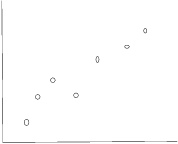
\includegraphics[width=0.3\textwidth]{FIG/data.png} &
     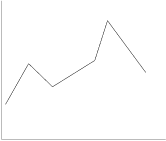
\includegraphics[width=0.3\textwidth]{FIG/plot.png} \\
     %\psfig{figure=FIG/plot.ps,width=2in} \\
     % \psfig{figure=FIG/data.ps,width=2in} &
     % \psfig{figure=FIG/plot.ps,width=2in} \\
    (a) & (b) 
\end{tabular}
\caption{A fictitious dataset (a) and its performance plot (b)}
\label{fig:results}
\end{center}
\end{figure}



\section{Conclusions}
    \label{sec:conclusions}
    The proposed method {\em someMETHOD}
has the following advantages:
\bit
\item it gives better classification accuracy than all 10 competitors we tried
\item its accuracy is very close to the very best competitor
      in the {\em UCR Insect Classification Contest}.
\item it is scalable
\eit



\bibliography{BIB/christosref,BIB/other}
\bibliographystyle{plain}

\newpage
\appendix
\section{Appendix}

\subsection{Labor Division}

The team performed the following tasks
\bit
\item Implementation of Daubechies-4 [Smith, Thompson]
\item Comparison of Daubechies-4 against euclidean distance [Miller]
\item Data collection [all]
\item Experiments on the real data [Miller]
\eit

\subsection{Full disclosure wrt dissertations/projects}

\paragraph{Smith:}
His dissertation  is on a music retrieval system ('query by whistle').
Although related to this class's project,
Smith never considered wavelets, AutoRegression, or generalized-time-warping,
for his dissertation, that he studied and implemented in this project.

\paragraph{Thompson:}
She is not doing any project or dissertation
related to this project: her thesis is on phylogenetic trees.

\paragraph{Miller:} He is not doing any project or dissertation
related to this project: his thesis is on dark matter discovery.


\newpage
\pagenumbering{roman}
\tableofcontents


\end{document}
